\section*{Seminár 21}
\subsection*{Téma}
Geometria V~-- štvoruholníky

\subsection*{Ciele}
Uplatniť znalosti z~predchádzajúcich geometrických seminárov pri riešení úloh o štvoruholníkoch.

\subsection*{Úlohy a riešenia}
\begin{tcolorbox}[breakable,notitle,boxrule=0pt,colback=light-gray,colframe=light-gray]\ul{21.1} [57-I-2] Štvoruholníku $ABCD$ je vpísaná kružnica so stredom $S$. Určte rozdiel $|\ma ASD|- |\ma CSD|$, ak $|\ma ASB| - |\ma BSC| = 40^\circ$

\end{tcolorbox}

\rieh Päty kolmíc spustených zo stredu $S$ vpísanej kružnice na strany $AB$, $BC$, $CD$ a $DA$ označme postupne $K$, $L$, $M$ a $N$ (obr. 1). Pravouhlé trojuholníky $ASK$ a $ASN$ sú zhodné podľa vety $Ssu$. Majú totiž spoločnú preponu $AS$ a zhodné odvesny $SK$ a $SL$, ktorých dĺžka je rovná polomeru vpísanej kružnice. Zo zhodnosti týchto trojuholníkov vyplýva jednak známe tvrdenie o~dĺžkach dotyčníc $(|AK| = |AN|)$, jednak zhodnosť uhlov $ASK$ a $ASN$, ktorých spoločnú veľkosť označíme~$\alpha$:$$|\ma ASK| = |\ma ASN| = \alpha.$$
\begin{center}
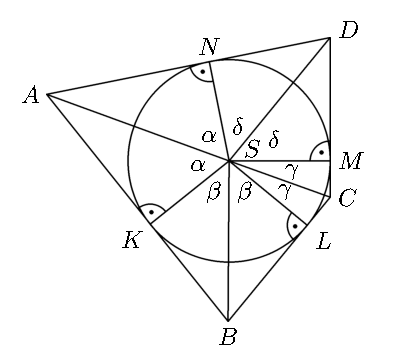
\includegraphics{obrazky/57D2}\\

Obr. 1
\end{center}
Analogicky zistíme zhodnosť trojuholníkov $SBK$ a $SBL$, ďalej $SCL$ a $SCM$, a nakoniec $SDM$ a $SDN$. Na základe uvedených zhodností môžeme položiť
$$|\ma BSK| = |\ma BSL| = \beta, \ \ \ \  |\ma CSL| = |\ma CSM| = \gamma, \ \ \ \  |\ma DSM| = |\ma DSN| = \delta.$$
Odtiaľ a z~obr. 1 potom dostávame
\begin{align*}
|\ma ASD| - |\ma CSD| &= (\alpha + \delta)- (\gamma + \delta) = \alpha - \gamma =\\
&= (\alpha + \beta) - (\gamma + \beta) = |\ma ASB| - |\ma BSC| = 40^\circ.
\end{align*}
\textit{Záver.} $|\ma ASD|  -|\ma CSD| = 40^\circ$.\\
\\
\kom Úloha je relatívne nezložitým úvodom do seminára a nadväzuje na posledné geometrické stretnutie, ktoré sa zaoberalo opísanými a vpísanými kružnicami trojuholníku. Pre úplnosť len dodajme, že štvoruholník, ktorému je možné vpísať kružnicu, sa nazýva \textit{dotyčnicový}.\\
\\
\begin{tcolorbox}[breakable,notitle,boxrule=0pt,colback=light-gray,colframe=light-gray]\ul{21.2} [61-II-3] Nech $E$ je stred strany $CD$ rovnobežníka $ABCD$, v~ktorom platí $2|AB| = 3|BC|$. Dokážte, že ak sa dá do štvoruholníka ABCE vpísať kružnica, dotýka sa táto kružnica strany $BC$ v~jej strede.

\end{tcolorbox}

\rieh Keďže štvoruholník $ABCE$ je podľa zadania dotyčnicový, pre dĺžky jeho strán platí známa rovnosť\footnote{Rovnosť sa odvodí rozpísaním dĺžok strán na ich úseky vymedzené bodmi dotyku vpísanej kružnice a následným využitím toho, že každé dva z~týchto úsekov, ktoré vychádzajú z~rovnakého vrcholu
štvoruholníka, sú zhodné.}
$$|AB| + |CE| = |BC| + |AE|.$$
V~našej situácii pri označení $a = |AB|$ platí $|BC| = |AD| = \frac{2}{3}a$ a $|CE| = |DE| =\frac{1}{2}a$
(obr. 2), odkiaľ po dosadení do uvedenej rovnosti zistíme, že $|AE| = \frac{5}{6}a$.
\begin{center}
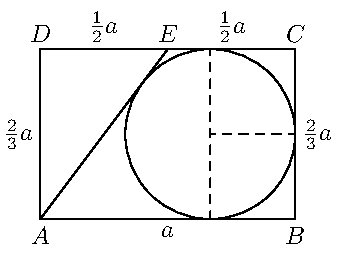
\includegraphics{obrazky/61K31}\\

Obr. 2
\end{center}
Teraz si všimneme, že pre dĺžky strán trojuholníka $ADE$ platí
$$|AD| : |DE| : |AE| = \frac{2}{3}a : \frac{1}{2}a : \frac{5}{6}a = 4 : 3 : 5,$$
takže podľa (obrátenej časti) Pytagorovej vety má trojuholník $ADE$ pravý uhol pri vrchole $D$, a teda rovnobežník $ABCD$ je obdĺžnik. Dotyčnica $BC$ kružnice vpísanej štvoruholníku $ABCE$ je teda kolmá na dve jej (navzájom rovnobežné) dotyčnice $AB$ a $CE$. To už zrejme znamená, že bod dotyku dotyčnice $BC$ je stredom úsečky $BC$ (vyplýva to zo zistenej kolmosti vyznačeného priemeru kružnice na jej vyznačený
polomer).\\
\\
\textbf{Iné riešenie.} Ukážeme, že požadované tvrdenie možno dokázať aj bez toho, aby sme si všimli, že rovnobežník $ABCD$ je v~danej úlohe obdĺžnikom. Namiesto toho využijeme, že úsečka $CE$ je stredná priečka trojuholníka $ABF$, pričom $F$ je priesečník polpriamok $BC$ a $AE$ (obr. 3), lebo $CE \parallel AB$ a $|CE| =\frac{1}{2}|AB|$. Označme preto $a = |AB| = 2|CE|$,
\begin{center}
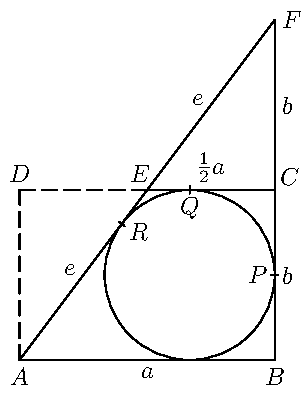
\includegraphics{obrazky/61K32}\\

Obr. 3
\end{center}
$b = |BC| = |CF|$ a $e = |AE| = |EF|$ (rovnosť $2a = 3b$ použijeme až neskôr). Rovnako ako v~prvom riešení využijeme rovnosť $b+e = a+\frac{1}{2}a (=\frac{3}{2}a)$, ktorá platí pre dĺžky strán dotyčnicového štvoruholníka $ABCE$. Kružnica jemu vpísaná sa dotýka strán $BC$, $CE$, $AE$ postupne v~bodoch $P$, $Q$, $R$ tak, že platia rovnosti
$$|CP| = |CQ|, \ \ \ \ |EQ| = |ER| \ \ \ \ \text{a tiež}\ \ \ \ |FP| = |FR|.$$
Pre súčet zhodných dĺžok $|FP|$ a $|FR|$ teda platí
\begin{align*}
|FP| + |FR| &= (b + |CP|) + (e + |ER|) = (b + e) + (|CP| + |ER|) =\\
&=\frac{3}{2}a + (|CQ| + |EQ|) = \frac{3}{2}a + \frac{1}{2}a = 2a,
\end{align*}
čo znamená, že $|FP| = |FR| = a$.

Teraz už riešenie úlohy ľahko dokončíme. Rovnosť $|BP| =\frac{1}{2}b$, ktorú máme v~našej situácii dokázať, vyplýva z~rovnosti
$$|BP| = |BF| - |FP| = 2b -a,$$
keď do nej dosadíme zadaný vzťah $a=\frac{3}{2}b$.\\
\\
\kom Úloha nadväzuje na predchádzajúcu a využíva rovnosť súčtov dĺžok opačných strán dotyčnicového štvoruholníka. Ďalej študenti uplatnia buď Pytagorovu vetu alebo vedomosti o~stredných priečkach v~trojuholníku, čo úlohu činí zaujímavou z~hľadiska pestrosti.\\
\\
\begin{tcolorbox}[breakable,notitle,boxrule=0pt,colback=light-gray,colframe=light-gray]\ul{21.3} [59-II-3]  Daná je kružnica $k$ so stredom $S$. Kružnica $l$ má väčší polomer ako kružnica $k$, prechádza jej stredom a pretína ju v~bodoch $M$ a $N$. Priamka, ktorá prechádza bodom $N$ a je rovnobežná s~priamkou $MS$, vytína na kružniciach tetivy $NP$ a $NQ$. Dokážte, že trojuholník $MPQ$ je rovnoramenný.

\end{tcolorbox}

\rieh Polomer kružnice $k$ označme $r$. Označenie vrcholov $P$, $Q$ v~trojuholníku $MPQ$ nie je dôležité, preto bez ujmy na všeobecnosti označme $P$ ten z~bodov priamky vedenej bodom $N$ rovnobežne s~priamkou $MS$, ktorý leží na kružnici $k$. Bod $Q$ potom leží na kružnici $l$ a štvoruholník $NQMS$ je lichobežník vpísaný do kružnice $l$ (obr. 4). Je teda rovnoramenný s~ramenami $MQ$ a $NS$ dĺžky $r$. Navyše aj úsečky $SP$ a $SM$ majú dĺžku $r$. Z~rovnoramenného trojuholníka $NPS$ a rovnoramenného lichobežníka $NQMS$ vyplýva rovnosť uhlov $|\ma SPN| = |\ma SNP| = |\ma MQP|$. Priečka $PQ$ teda pretína priamky $SP$ a $MQ$ pod rovnako veľkými uhlami, a preto (podľa vety o~súhlasných uhloch) sú priamky $SP$ a $MQ$ rovnobežné. Štvoruholník $PQMS$ je teda rovnobežník, a keďže $|SM| = |SP| = r$, je to dokonca kosoštvorec. Odtiaľ je už zrejmé, že trojuholník $MPQ$ je rovnoramenný s~ramenami $PQ$ a $MQ$ dĺžky $r$.
\begin{center}
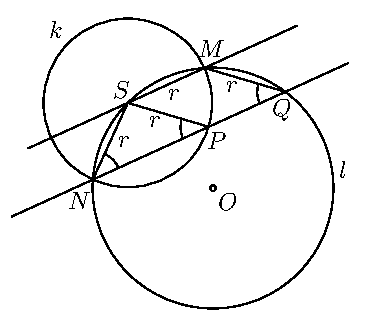
\includegraphics{obrazky/59K31}\\

Obr. 4
\end{center}
\textit{Poznámka.} Existencia tetív $NP$ a $NQ$ v~zadaní je zaručená vďaka predpokladu, že kružnica $l$ má väčší polomer ako kružnica $k$. Ak označíme $C$ stred úsečky $SM$ a $E$ ten priesečník kružnice $k$ s~osou úsečky $SM$, ktorý leží v~polrovine $SMO$, bude stred O~kružnice $l$ ležať na polpriamke $CE$ až za bodom $E$ (obr. 5). Ďalší priesečník $N$ oboch
\begin{center}
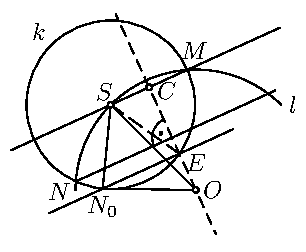
\includegraphics{obrazky/59K32}\\

Obr. 5
\end{center}
kružníc preto padne do pásu medzi rovnobežkami $SM$ a $N_0 E$ v~polrovine $OCS$, pričom $N_0$ je štvrtý vrchol kosoštvorca s~vrcholmi $S$, $M$, $E$. Na to stačí ukázať, že kružnica $l$ pretne polpriamku $EN_0$ až za bodom $N_0$, teda že jej polomer $OS$ je väčší ako dĺžka úsečky $ON_0$. Toto porovnanie dvoch strán trojuholníka $OSN_0$ jednoducho vyplýva z~porovnania jeho vnútorných uhlov: uhol pri vrchole $N_0$ je najväčší, lebo oba uhly pri protiľahlej strane $OS$ sú menšie ako $60^\circ$ (trojuholník $ESN_0$ je rovnostranný). Ľahko nahliadneme, že každá z~rovnobežiek uvedeného pásu pretína každú z~oboch kružníc v~dvoch bodoch (vždy súmerne združených podľa príslušnej osi kolmej na $SM$). Tým je dokázaná nielen existencia oboch tetív $NP$ a $NQ$, ale aj to, že ich krajné body $P$ a $Q$ ležia na rovnakej strane od bodu $N$ (ako na obr. 4), lebo oba body zrejme ležia v~polrovine opačnej k~spomenutej polrovine $OCS$.\\
\\
\kom Diskusia v~poznámke je len zaujímavým doplnkom úlohy, existencia tetív je totiž predpokladom zadania a nie je nutné ju dokazovať. Úloha využíva úvahu, že lichobežník, ktorého základne sú rovnobežné tetivy danej kružnice, je rovnoramenný, ktorá môže byť pre študentov zaujímavým uvedomením.\\
\\
\begin{tcolorbox}[breakable,notitle,boxrule=0pt,colback=light-gray,colframe=light-gray]\ul{21.4} [60-I-3]  Máme štvorec $ABCD$ so stranou dĺžky 1\,cm. Body $K$ a $L$ sú stredy strán $DA$ a $DC$. Bod $P$ leží na strane $AB$ tak, že $| BP | = 2 | AP |$. Bod $Q$ leží na strane $BC$ tak, že $| CQ | = 2 | BQ |$. Úsečky $KQ$ a $PL$ sa pretínajú v~bode $X$. Obsahy štvoruholníkov $APXK$, $BQXP$, $QCLX$ a $LDKX$ označíme postupne $S_A$, $S_B$, $S_C$, $S_D$ (obr. 6).

a) Dokážte, že $S_B = S_D$.

b) Vypočítajte rozdiel $S_C - S_A$.

c) Vysvetlite, prečo neplatí $S_A + S_C = S_B + S_D$.
\begin{center}
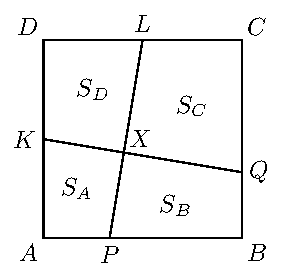
\includegraphics{obrazky/60D31}\\

Obr. 6
\end{center}
\end{tcolorbox}

\rieh  a) Štvoruholníky $ABQK$ a $DAPL$ sú zhodné (jeden z~nich je obrazom druhého v~otočení o~$90^\circ$ so stredom v~strede štvorca $ABCD$). Preto majú aj rovnaký obsah, čiže $S_A + S_B = S_A + S_D$. Z~toho hneď dostaneme $S_B = S_D$.

b) Ľahko sa nám podarí vypočítať obsah pravouhlého lichobežníka $ABQK$, lebo poznáme dĺžky základní aj výšku. Dostaneme
$$S_A + S_B =\bigg( \frac{1}{2}+\frac{1}{3}\bigg)\cdot \frac{1}{2}=\frac{5}{12}\,\text{cm}^2.$$
Podobne výpočtom obsahu lichobežníka $PBCL$ dostaneme
$$S_C + S_B =\bigg(\frac{1}{2}+\frac{2}{3}\bigg)\cdot\frac{1}{2}=\frac{7}{12}\,\text{cm}^2.$$
Odčítaním prvej získanej rovnosti od druhej dostávame $S_C - S_A =\frac{7}{12}-\frac{5}{12}=\frac{1}{6}\,\text{cm}^2$.

c) Nerovnosť medzi obsahmi $S_A + S_C$ a $S_B + S_D$ (ktorých priame výpočty nie sú v~silách žiakov 1. ročníka) môžeme zdôvodniť nasledovným spôsobom: Súčet týchto dvoch obsahov je 1\,cm$^2$, takže sa nerovnajú práve vtedy, keď je jeden z~nich menší ako $\frac{1}{2}$\,cm$^2$. Bude to obsah $S_B +S_D$ (rovný $2S_B$, ako už vieme), keď ukážeme, že obsah $S_B$ je menší ako $\frac{1}{4}$\,cm$^2$. Urobíme to tak, že do celého štvorca $ABCD$ umiestnime bez prekrytia štyri kópie štvoruholníka $PBQX$. Ako ich umiestnime, vidíme na obr. 7, pričom $M$, $N$ sú stredy strán $BC$, $AB$ a $R$, $S$ body, ktoré delia strany $CD$, $DA$ v~pomere $1 : 2$.
\begin{center}
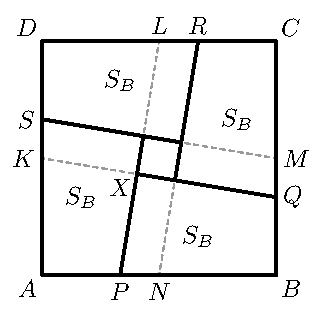
\includegraphics{obrazky/60D32} 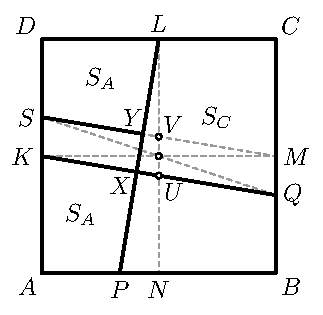
\includegraphics{obrazky/60D33}\\

Obr. 7 \hspace{140pt} Obr. 8
\end{center}
\textbf{Iné riešenie} časti c). Tentoraz namiesto nerovnosti $S_B + S_ D < \frac{1}{2}$\,cm$^2$ dokážeme ekvivalentnú nerovnosť $S_A +S_C >\frac{1}{2}$\,cm$^2$. Preto sa pokúsime \uv{premiestniť} štvoruholník $APXK$ tak, aby ležal pri štvoruholníku $XQCL$ a aby sa ich obsahy dali geometricky sčítať. Uhly $AKQ$ a $DLP$ sú zhodné a $| AK | = | DL |$, preto môžeme štvoruholník $APXK$ premiestniť vo štvorci $ABCD$ do jeho \uv{rohu} $D$ tak, že k~štvoruholníku $XQCL$ priľahne pozdĺž strany $LX$ svojou stranou $LY$, pričom $Y$ je priesečník úsečiek $SM$ a $PL$ z~pôvodného riešenia (obr. 8). Obsah $S_A + S_C$ je potom obsahom šesťuholníka $DSYXQC$. Prečo je väčší ako $\frac{1}{2}$\,cm$^2$, môžeme zdôvodniť napríklad takto:

Úsečka spájajúca bod $L$ so stredom $U$ úsečky $KQ$ pretne úsečku $SM$ v~jej strede $V$. Štvoruholník $UQMV$ má obsah rovný polovici obsahu rovnobežníka $KQMS$, teda rovný obsahu trojuholníka $KMS$. Preto má šesťuholník $DSV UQC$ obsah rovný obsahu štvoruholníka $KMCD$,  t.\,j. polovici obsahu štvorca $ABCD$. Obsah $S_A +S_C$ je ešte väčší, a to o~obsah štvoruholníka $XUVY$. Teda naozaj $S_A + S_C >\frac{1}{2}$\,cm$^2$.\\
\\
\kom Prvé dve časti sú príjemným úvahovým rozohriatím k~časti tretej, ktorá vyžaduje trochu viac invencie. Demonštruje však zaujímavý prístup k~riešeniu a porovnávanie obsahov obrazcov namiesto priameho výpočtu obsahov.\\
\\
\begin{tcolorbox}[breakable,notitle,boxrule=0pt,colback=light-gray,colframe=light-gray]\ul{21.5} [66-I-5-prvá časť] Ak označíme $X$ a $Y$ postupne stredy základní $RS$ a $TU$ všeobecného lichobežníka $RSTU$, tak na úsečke $XY$ leží priesečník $P$ uhlopriečok $RT$ a $SU$, a to tak, že $|PX| : |PY | = |RS| : |TU|$. Na priamke $XY$ leží tiež priesečník $Q$ predĺžených ramien $RU$ a $ST$, a to tak, že $|QX| : |QY | = |RS| : |TU|$ (obr. 9). Dokážte.

\end{tcolorbox}

\rieh
\begin{center}
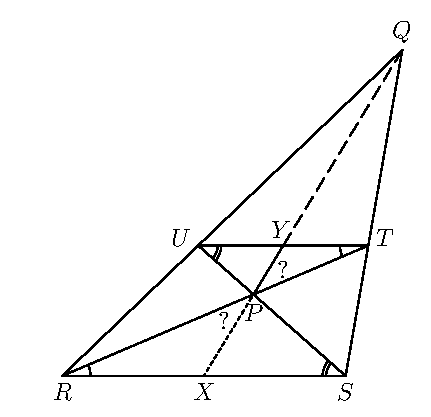
\includegraphics{obrazky/66D51}\\

Obr. 9
\end{center}
Napriek tomu, že sa podľa obrázka zdá, že bod $P$ na úsečke $XY$ naozaj leží, musíme tento poznatok dokázať, teda \textit{odvodiť} argumentáciou nezávislou na presnosti nášho rysovania. Na to určite stačí preukázať, že obe úsečky $PX$, $PY$ zvierajú s~priamkou $RT$ zhodné uhly (na obrázku vyznačené otáznikmi). Všimnime si, že tieto úsečky sú ťažnicami trojuholníkov $RSP$ a $TUP$, ktoré sa zhodujú vo vnútorných uhloch (vyznačených oblúčikmi) pri rovnobežných stranách $RS$ a $TU$, takže ide o~trojuholníky podobné, a to s~koeficientom $k = |TU|/|RS|$. S~rovnakým koeficientom platí aj podobnosť \uv{polovíc} týchto trojuholníkov vyťatých ich ťažnicami, presnejšie podobnosť $RXP \sim TYP$. Z~nej už želaná zhodnosť uhlov $RPX$ a $TPY$ aj želaná rovnosť $|PY | = k|PX|$ (vďaka rovnakému koeficientu) vyplýva. Všetko o~bode $P$ je tak dokázané; podobne sa overia aj obe vlastnosti bodu $Q$ - ukáže sa, že úsečky $QX$ a $QY$ zvierajú ten istý uhol s~priamkou $RQ$ a ich dĺžky sú zviazané rovnosťou $|QY | = k|QX|$, a to vďaka tomu, že $QX$ a $QY$ sú ťažnice v~dvoch navzájom podobných trojuholníkoch $RSQ$ a $UTQ$.\\
\\
\kom Úloha je prípravou na riešenie záverečného problému tohto seminára a pripomína študentom metódu dôkazu toho, že bod $P$ leží na priamke úsečke $XY$.\\
\\
\begin{tcolorbox}[breakable,notitle,boxrule=0pt,colback=light-gray,colframe=light-gray]\ul{21.6} [66-I-5] V~danom trojuholníku ABC zvoľme vnútri strany $AC$ body $K$, $M$ a vnútri strany $BC$ body $L$, $N$ tak, že
$$|AK| = |KM| = |MC|, |BL| = |LN| = |NC|.$$
Ďalej označme $E$ priesečník uhlopriečok lichobežníka $ABLK$, $F$ priesečník uhlopriečok lichobežníka $KLNM$ a $G$ priesečník uhlopriečok lichobežníka $ABNM$. Dokážte, že body $E$, $F$ a $G$ ležia na ťažnici trojuholníka $ABC$ z~vrcholu $C$ a určte pomer $|GF| : |EF|$.

\end{tcolorbox}

\rieh
Dokázané vlastnosti všeobecného lichobežníka z~predchádzajúcej úlohy nám umožnia celkom ľahko vyriešiť zadanú úlohu. Situácia je znázornená na obr. 10. Okrem pomenovaných bodov sme tam ešte označili $S_1$, $S_2$, $S_3$ stredy úsečiek $AB$, $KL$ a $MN$. Keďže trojuholníky $ABC$, $KLC$
\begin{center}
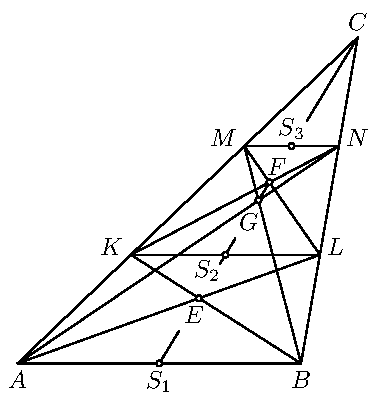
\includegraphics{obrazky/66D52}

Obr. 10
\end{center}
a $MNC$ sú navzájom podobné (podľa vety $sus$), platí $|AB| : |KL| : |MN| = |AC| : |KC| : |MC| = 3 : 2 : 1$. Podľa zhodných vnútorných uhlov spomenutých troch trojuholníkov platí tiež $AB \parallel KL$, $KL \parallel MN$. Štvoruholníky $ABLK$, $KLNM$ a $ABNM$ tak sú naozaj lichobežníky (ako je prezradené v~zadaní) so základňami $AB$, $KL$ a $MN$, ktorých dĺžky sú v~už odvodenom pomere $3 : 2 : 1$. Navyše predĺžené ramená všetkých troch lichobežníkov sa pretínajú v~bode $C$, ktorým preto podľa dokázanej vlastnosti prechádzajú priamky $S_1 S_2$, $S_2 S_3$ (a $S_1 S_3$), takže ide o~jednu priamku, na ktorej body $S_1$, $S_2$, $S_3$ a $C$ ležia v~uvedenom poradí tak, že $|S_1 C| : |S_2 C| : |S_3 C| = 3 : 2 : 1$. Z~toho vyplýva $|S_1 S_2 | = |S_2 S_3 | (= |S_3 C|)$, takže bod $S_2$ je stredom úsečky $S_1 S_3$. Na nej (opäť podľa dokázaného tvrdenia) ležia aj body $E$, $F$ a $G$, pričom pre bod $E$ medzi bodmi $S_1$, $S_2$ platí $|ES_1 | : |ES_2 | = 3 : 2$, pre bod $F$ medzi bodmi $S_2$, $S_3$ platí $|FS_2| : |FS_3| = 2 : 1$ a napokon pre bod $G$ medzi bodmi $S_1$, $S_3$ platí $|GS_1| : |GS_3 | = 3 : 1$. Tieto delenia troch úsečiek sme znázornili na obr. 11, kam sme zapísali aj dĺžky vzniknutých úsekov pri voľbe jednotky $1 = |S_1 S_2 | = |S_2 S_3 |$ (pri ktorej $|S_1 S_3 | = 2$).
\begin{center}
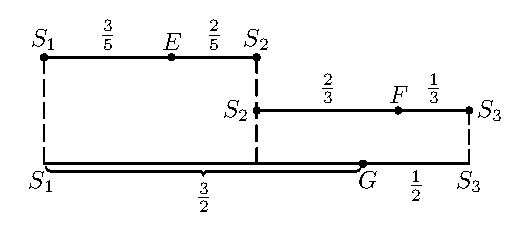
\includegraphics{obrazky/66D53}

Obr. 11
\end{center}
Keďže
$$|S_1 F| = |S_1 S_2 | + |S_2 F| = 1 +\frac{2}{3}=\frac{5}{3}>\frac{3}{2}= |S_1 G|,$$
platí $|GF| = |S_1 F| - |S_1 G| =\frac{5}{3} -\frac{3}{2}=\frac{1}{6}$, čo spolu s~rovnosťou $|EF| = |ES_2 | + |S_2 F|=\frac{2}{5}+\frac{2}{3}=\frac{16}{15}$ už vedie k~určeniu hľadaného pomeru
$$|GF| : |EF| =\frac{1}{6}:\frac{16}{15}= 5 : 32.$$
\\
\kom Úloha je zložitejšia ako predchádzajúca, ale študenti zoznámení s~prípravnou úlohou, zbehlí vo využívaní podobných trojuholníkov a precízni, aby sa nestratili v~záverečnom pomerovaní, by si s~úlohou poradiť mali.
